%-------------------------------------------------------------------------------
%-------------------------------------------------------------------------------
%-------------------------------------------------------------------------------
\chapter{X 2021}
%-------------------------------------------------------------------------------
%-------------------------------------------------------------------------------
\vskip -2cm
\begin{center}
    \Huge \bf Facteurs dans les mots binaires
\end{center}
%-------------------------------------------------------------------------------
%-------------------------------------------------------------------------------
%-------------------------------------------------------------------------------
\section{Arbres de mots}
%-------------------------------------------------------------------------------
%-------------------------------------------------------------------------------
%-------------------------------------------------------------------------------
\begin{Exercise}
\begin{minipage}{0.5\textwidth}
L'arbre $a_2$ représente $\{00, 1, 101\}$.

L'ensemble $\{\varepsilon, 00,010, 1, 110, 111\}$ est représenté par l'arbre ci-contre.
\end{minipage}
\begin{minipage}{0.5\textwidth}
\begin{center}
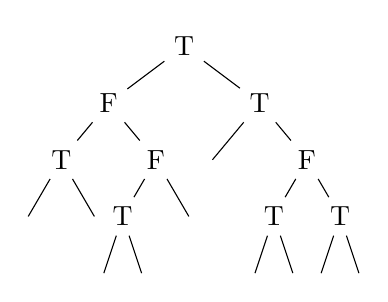
\begin{tikzpicture}[level distance =12mm, scale = 0.6]
  \tikzstyle{level 1}=[sibling distance =32mm]
  \tikzstyle{level 2}=[sibling distance =20mm]
  \tikzstyle{level 3}=[sibling distance =14mm]
  \tikzstyle{level 4}=[sibling distance =8mm]
%  \tikzstyle{every node}=[circle,draw]
  \node  {T}
   child {node{F}
          child {node{T}
                 child [fill=none] 
                 child [fill=none] 
                }
          child {node{F}
                 child {node{T}
                        child [fill=none]
                        child [fill=none]
                       }
                 child [fill=none]
                }
         }
   child {node {T}
          child [fill=none]
          child {node{F}
                 child {node{T}
                        child [fill=none]
                        child [fill=none]
                       }
                 child {node{T}
                        child [fill=none]
                        child [fill=none]
                       }
                }
        };
\end{tikzpicture}    
\end{center}
\end{minipage}
\end{Exercise} 
%-------------------------------------------------------------------------------
%-------------------------------------------------------------------------------
\begin{Exercise}
On commence par le cas de l'ensemble vide 
\begin{enumerate}
    \item $\emptyset$ est représenté par l'arbre vide.
    \item Pour montrer l'unicité de l'arbre réduit représentant $\emptyset$ on va montrer que l'ensemble vide ne peut être représenté que par un arbre vide ou un arbre ne contenant que des nœuds de valeur \type{false}.
    \item Pour cela on montre par récurrence sur la profondeur d'un nœud de valeur \type{true}que si un arbre contient un nœud de valeur \type{true} alors il ne représente pas l'ensemble vide.
    \begin{itemize}
        \item Si la racine a la valeur \type{true} alors l'ensemble représenté contient $\varepsilon$ donc il est non vide.
        \item On suppose la propriété est vraie pour un nœud à la profondeur $p$. Pour un arbre contenant un nœud de valeur \type{true} à la profondeur $p+1$, un de ses fils contient ce nœud à la profondeur $p$ donc représente un ensemble $M$ non vide et l'arbre initial représente un ensemble contenant $\{0m\; m\in M\}$ donc un ensemble non vide.
    \end{itemize}
    \item On en déduit qu'un non vide représentant l'ensemble vide ne contient que des nœuds de valeur \type{false} : ses nœuds terminaux sont donc de la forme $N(\type{false}, V, V)$ : il ne peut pas être réduit.
Ainsi l'ensemble vide est représenté par un unique arbre réduit, l'arbre vide.
\end{enumerate}
\medskip

Pour prouver ensuite que tout ensemble est représenté par un unique arbre réduit on va procéder par récurrence sur la longueur maximale d'un mot de cet ensemble qu'on nommera la {\bf longueur} de l'ensemble.

Soit ${\cal P}(n)$ la propriété : pour tout langage vide ou de longueur strictement inférieure à $n$, il existe un unique arbre de mots réduit qui le représente.
\begin{itemize}
    \item ${\cal P}(0)$ ne concerne que $\emptyset$ pour lequel on a prouvé l'existence et l'unicité de l'arbre réduit le représentant.
    \item On suppose ${\cal P}(n)$ vérifiée ; pour prouver ${\cal P}(n+1)$ il reste à prouver la propriété pour les ensembles de longueur $n$.
    
    Soit $E$ un ensemble de longueur $n$,  on le décompose en 3 parties : $E_r = E\cap \{\varepsilon\}$, $E_g$ (resp. $E_d$) est l'ensemble des mots de $E$ qui commencent par 0 (resp. par 1).
    
    On peut écrire $E_g = \{0m\ ;\ m\in E'_g\}$ où $E'_g\}$ est l'ensemble des mots de $E_g$ privés de leur première lettre 0 ; de même $E_d = \{1m\ ;\ m\in E'_d\}$.
    
    Pour construire un arbre qui représente $E$ on doit l'écrire $N(b, g, d)$ avec $b$ valant \type{true} ou \type{false} selon que $E_r=\{\varepsilon\}$ ou $E_r=\emptyset$ et $g$ et $d$ sont des arbres représentant respectivement $E'_g$ et $E'_d$. Comme $E'_g$ et $E'_d$ sont vides ou de longueur au plus $n-1$, l'hypothèse de récurrence permet de construire $g$ et $d$ réduits et de manière unique. 
    
    L'arbre $N(b, g, d)$ n'est alors pas réduit. En effet, en dehors de la racine, les nœuds sont des nœuds de $g$ ou de $d$ distincts de $N(\type{false}, V, V)$ car $g$ et $d$ sont réduits.
    
    La racine non plus ne peut pas être $N(\type{false}, V, V)$ car cela impliquerait $E_0=E_g=E_d=\emptyset$ donc $E = \emptyset$, impossible pour un ensemble de longueur $n$ donc non vide.
\end{itemize}
\end{Exercise} 
%-------------------------------------------------------------------------------
%-------------------------------------------------------------------------------
\begin{Exercise}À gauche de la racine, on doit représenter les mots de longueur $n-1$, à droite, seulement $1^{n-1}$.
\begin{lstlisting}
let rec uns n =
   if n = 0
   then N(true, V, V)
   else N(false, V, uns (n-1));;
\end{lstlisting}
\begin{lstlisting}
let rec zeros_puis_uns n =
   if n = 0
   then N(true, V, V)
   else N(false, zeros_puis_uns (n-1), uns (n-1));;
\end{lstlisting}
\end{Exercise} 
%-------------------------------------------------------------------------------
%-------------------------------------------------------------------------------
\begin{Exercise}Si $k = 0$, on représente tous les mots $0^p$, $0\le p \le n$
\begin{lstlisting}
let rec zeros n =
   if n = 0
   then N(true, V, V)
   else N(true, zeros (n-1), V);;
\end{lstlisting}
Si $k=n$ on représente $1^n$, comme ci-dessus et sinon on représente les mots de longueur au plus $n-1$ avec $k$ uns à gauche et les mots de longueur au plus $n-1$ avec $k-1$ uns à droite.
\begin{lstlisting}
let rec k_uns k n = 
   match n-k, k with
   |0, _ -> uns k
   |_, 0 -> zeros n
   |_ -> N(false, k_uns k (n-1), k_uns (k-1) (n-1));;
\end{lstlisting}
Je ne comprends pas l'indication de l'énoncé.
\end{Exercise} 
%-------------------------------------------------------------------------------
%-------------------------------------------------------------------------------
\begin{Exercise}
\begin{lstlisting}
let rec compter arbre =
   match arbre with
   |V -> 0
   |N(b, g, d) ->  (if b then 1 else 0) 
                  + compter g + compter d;;
\end{lstlisting}
\end{Exercise} 
%-------------------------------------------------------------------------------
%-------------------------------------------------------------------------------
\begin{Exercise}Aucun mot (même vide) ne peut être représenté par un arbre vide. Quand on a lu toutes les lettres, on doit tomber su un nœud de valeur \type{true}. Auparavant on a parcouru l'arbre à droite ou à gauche selon la valeur de \type{m.(i)}.
\begin{lstlisting}
let chercher arbre mot = 
   let n = Array.length mot in
   let rec aux_ch i a =
      match a with
      |V -> false
      |N(b, g, d) -> if i = n
                     then b 
                     else (if mot.(i) = 0
                           then aux_ch (i+1) g
                           else aux_ch (i+1) d) 
   in aux_ch 0 arbre;;              
\end{lstlisting}
\end{Exercise} 
%-------------------------------------------------------------------------------
%-------------------------------------------------------------------------------
\begin{Exercise}Le sujet est assez directif ici.
\begin{lstlisting}
let enumerer arbre = 
   let rec aux acc pref t =
      match t with
      |V -> acc
      |N(b, g, d) -> let acc1 = aux acc (0::pref) g in
            if b then let m = Array.of_list (List.rev pref) in 
                      aux (m::acc1) (1::pref) d
                 else aux acc1 (1::pref) d
      in aux [] [] arbre;;
\end{lstlisting}
Il y a un appel récursif pour chaque nœud de l'arbre.

Lors de chaque appel on effectue au plus 3 ajouts de termes dans une liste et on peut créer un nouveau mot qui sera placé dans la liste des mots. Cette création demande 2 opérations de complexité linéaire en la taille du mot.

La complexité globale est donc un ${\cal O}(n1 + n2)$ où $n_1$ est la taille de l'arbre et $n_2=\sum_{m \in {\mathbb M}(a)}\ell(m)$ est la somme des longueur des mots. Chaque nœud non vide (sauf la racine) correspond à une lettre d'au moins un mot car l'arbre est réduit donc, lorsque l'on parvient à un nœud terminal, avec la valeur \type{true}, on construit un mot dont la longueur est les nombre de nœuds visités. On a le nombre de nœuds non vides est donc majoré par $n_2+1$ (1 pour la racine) donc $n1={\cal O}( n2)$. On en déduit que la complexité est bien un ${\cal O}( n2)$
\end{Exercise} 
%-------------------------------------------------------------------------------
%-------------------------------------------------------------------------------
\begin{Exercise}On suit l'arbre tant que l'on peut puis on ajoute les nœuds si besoin. 

\newpage
\begin{lstlisting}
let ajouter arbre mot =
   let n  = Array.length mot in
   let rec aux a k =
      match arbre with
      |V -> if k = n
            then N(true, V, V)
            else begin if mot.(k) = 0
                       then N(false, aux V (k+1), V)
                       else N(false, V, aux V (k+1)) end
      |N(b, g, d) -> if k = n
                     then N(true, g, d)
                     else begin if mot.(k) = 0
                                then N(b, aux g (k+1), d)
                                else N(b, g, aux d (k+1)) end
   in aux arbre 0;;
\end{lstlisting}
\end{Exercise} 
%-------------------------------------------------------------------------------
%-------------------------------------------------------------------------------
%-------------------------------------------------------------------------------
\section{Arbre des suffixes}
%-------------------------------------------------------------------------------
%-------------------------------------------------------------------------------
%-------------------------------------------------------------------------------
\begin{Exercise}
\begin{center}
\begin{tikzpicture}[level distance =12mm, scale = 0.6]
  \tikzstyle{level 1}=[sibling distance =48mm]
  \tikzstyle{level 2}=[sibling distance =22mm]
  \tikzstyle{level 3}=[sibling distance =14mm]
  \tikzstyle{level 4}=[sibling distance =8mm]
%  \tikzstyle{every node}=[circle,draw]
  \node  {T}
   child {node{F}
          child [fill=none] 
          child {node{F}
                 child [fill=none]
                 child {node{T}
                        child [fill=none]
                        child [fill=none]
                       }
                }
         }
   child {node {T}
          child {node{F}
                 child [fill=none]
                 child {node{F}
                        child [fill=none]
                        child {node {T}
                               child [fill=none]
                               child [fill=none]
                              }
                       }
                }
          child {node{T}
                 child [fill=none]
                 child [fill=none]
                }
        };
\end{tikzpicture}    
\end{center}
\end{Exercise} 
%-------------------------------------------------------------------------------
%-------------------------------------------------------------------------------
\begin{Exercise}
Le mot $m$ est le plus long suffixe de $m$. Les nœuds non vides terminaux ont une valeur \type{true} et correspondent à des mots de l'arbre. Ainsi le nœud terminal correspondant à $m$ est à la profondeur maximale : $\ell(m)$. $\mathbb{AS}(m)$ est de hauteur $\ell(m)$.

\medskip
Pour déterminer le mot $m$ dans $\mathbb{AS}(m)$ il suffit donc de trouver le mot de l'arbre de longueur maximale. On écrit une fonction auxiliaire qui renvoie le mot le plus long et sa longueur.
\begin{lstlisting}
let retrouver_mot arbre =
   let rec rm_aux a =
      match a with
      |V -> [], -1
      |N(true, V, V) -> [], 0
      |N(false, V, V) -> failwith "L'arbre n'est pas réduit"
      |N(_, g, d) -> let m1, n1 = rm_aux g in
                     let m2, n2 = rm_aux d in
                     if n1 < n2 
                     then 1::m2, (1+n2)
                     else 0::m1, (1+n1)
   in Array.of_list (fst (rm_aux arbre));;   
\end{lstlisting}
\end{Exercise} 
%-------------------------------------------------------------------------------
\newpage
%-------------------------------------------------------------------------------
\begin{Exercise}
Les nœuds de $\mathbb{AS}(m)$ correspondent aux préfixes des mots de l'arbre donc aux préfixes des suffixes de $m$, c'est-à-dire aux facteurs de $m$.

\medskip

Un mot de longueur $n$ admet au moins un facteur de longueur $k$ pour tout $k\in \{0, 1, \ldots, n\}$ donc $n\bigl(\mathbb{AS}(m)\bigr)\ge \ell(m) +1$. Cette borne est atteinte pour le mot $[0; 0; \cdots; 0]$ de longueur $n$ qui a exactement $n+1$ facteur. Dans ce cas $\mathbb{AS}(m)$ est un arbre linéaire.

\medskip

Un facteur d'un mot $m$ est $m[i..j[$ avec $0\le i \le j \le \ell(m)$. Le nombre de facteurs non vides est donc majoré par le nombre de couples $(i,j)$ avec $0\le i < j \le \ell(m)$ : il y en a $\frac 12\ell(m)\bigl(\ell(m) + 1\bigr)$ ; en ajoutant le facteur vide on trouve donc un nombre de facteurs au plus quadratique.

Pour déterminer un mot avec "beaucoup" de facteurs on va considérer $m=0^p1^p$.

\begin{itemize}
    \item Pour $0\le k \le p$, $m$ a $k+1$ facteurs de longueur $k$ : $0^i1^{k-i}$ pour $0\le i \le k$.
    \item Pour $p< k \le \ell(m) = 2p$, $m$ a $2p-k+1$ facteurs de longueur $k$ : $0^{i+k-p}1^{p-i}$ pour $0\le i \le 2p-k$ car un facteur de longueur $k > p$ contient au moins $k-p$ lettres 0 et $k-p$ lettres 1.
    \item Le nombre de facteurs de $m$ est 
$\displaystyle \sum_{k=0}^p (k+1) +\sum_{k=p+1}^{2p} (2p-k+1)
=\sum_{i=1}^{p+1} i + \sum_{i=1}^{p}i
= p^2 = \frac{\bigl(\ell(m)\bigr)^2}4$.
\end{itemize}
Ainsi, pour toute longueur $\ell$ (paire), il existe un mot $m$ de longueur $\ell$ tel que $\mathbb{AS}(m)$ a $\frac{\ell^2}4$ nœuds.
\end{Exercise} 
%-------------------------------------------------------------------------------
%-------------------------------------------------------------------------------
%-------------------------------------------------------------------------------
\section{Arbre des facteurs}
%-------------------------------------------------------------------------------
%-------------------------------------------------------------------------------
%-------------------------------------------------------------------------------
\begin{Exercise}
$\mathbb{M}(a_5)=\{\varepsilon, 1, 001, 1001, 01001\}$, $a_5$ n'est pas un arbre des facteurs de $m$.

$\mathbb{M}(a_6)=\{\varepsilon, 1, 0, 1 001, 1001, 01001\}$, $a_6$ est un arbre des facteurs réduit de $m$.

$\mathbb{M}(a_7)=\{\varepsilon, 1, 0, 1 001, 1001, 01001\}$, $a_7$ est un arbre des facteurs non réduit de $m$.
\end{Exercise} 
%-------------------------------------------------------------------------------
%-------------------------------------------------------------------------------
\begin{Exercise}
\begin{enumerate}
    \item Comme l'arbre est réduit, tout nœud ayant au moins un fils vide a la valeur \type{true}. Or tout nœud de valeur \type{true} est associé à un suffixe, il y en a donc au plus $\ell(m)+1$. Comme le mot contient la lettre 0 et la lettre 1, il y a un suffixe qui commence par 0 et un suffixe qui commence par 1 ; on en déduit que la racine de l'arbre a deux fils non vides. Ainsi le suffixe $\varepsilon$ est associé à un nœud a deux fils non vides. Il y a donc au plus $\ell(m)$ nœuds ayant au moins un fils vide.
    \item Les sous-arbres vides sont les extrémités des nœuds ayant au moins un fils vide, il y a au plus $\ell(m)$ tels nœuds, chacun ayant au plus deux fils vides. On en déduit qu'il y a au plus $2\ell(m)$ sous-arbres vides. 
    
    Or on sait que le nombre de nœuds est égal au nombre de feuilles vides diminué de 1 donc un arbre de facteurs réduits pour le mot $m$ admet au plus $2\ell(m)-1$ nœuds.
    
    L'arbre des suffixes de $m=01$ est $e_1$ :

\begin{center}
\begin{tikzpicture}[level distance =12mm, scale = 0.6]
  \tikzstyle{level 1}=[sibling distance =32mm]
  \tikzstyle{level 2}=[sibling distance =18mm]
  \tikzstyle{level 3}=[sibling distance =14mm]
%  \tikzstyle{every node}=[circle,draw]
  \node  {T}
   child {node{F}
          child[fill=none]
          child {node{T}
                 child [fill=none]
                 child [fill=none]
                }
         }
   child {node {T}
          child [fill=none]
          child [fill=none]
         };
\end{tikzpicture}    
\end{center}
     On construit alors, par récurrence, $e_{k+1}=\type{N(true,} e'_k\type{, N(true, V, V))}$ où $e'_k$ est est obtenu à partir de $e_k$ en remplaçant la valeur de la racine par \type{false}.
     
     $e_k$ est l'arbre des suffixes de $0^k1$.
     
     Pour obtenir un un arbre des facteurs réduit il suffit de remplacer le nœud le plus à gauche par \type{N(k, k+1, T, V, V)} en éliminant son fils droit et d'ajouter la paire d'entiers 0, 0 à tous autres nœuds.
     
     Comme $e_k$ contient $2k+2$ nœuds, l'arbre de facteurs construit contient $2k+1$ nœuds, avec $2k+1 = 2\ell -1 $ pour $\ell = k+1$ égal à la longueur de $0^k1$.
    
    On représente l'arbre des facteurs associé à $e_5$ sans les fils vides.
    
\begin{center}
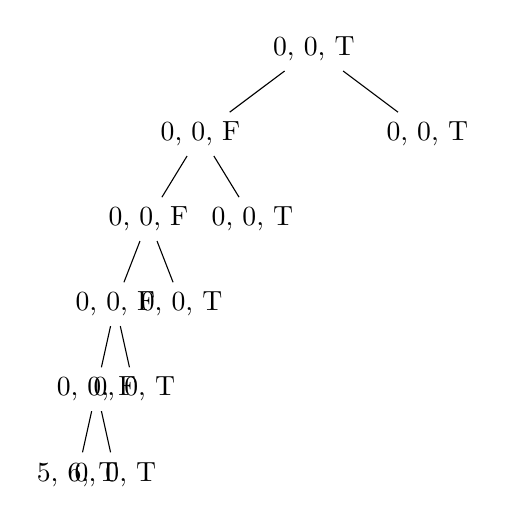
\begin{tikzpicture}[level distance =18mm, scale = 0.6, sibling distance = 32mm]
  \node{0, 0, T}
   child{node{0, 0, F}
         child{node{0, 0, F}
               child{node{0, 0, F}
                     child{node{0, 0, F}
                           child{node{5, 6, T}}
                           child{node{0, 0, T}}
                          }
                     child{node{0, 0, T}}
                    }
               child{node{0, 0, T}}
              }
         child {node{0, 0, T}}
        }
   child{node{0, 0, T}};
\end{tikzpicture}    
\end{center}
\end{enumerate}
\end{Exercise} 
%-------------------------------------------------------------------------------
%-------------------------------------------------------------------------------
\begin{Exercise}
On a vu que le nombre de facteurs était la taille de $\mathbb{AS}(m)$.

Dans le cas de l'arbre des facteurs, un nœud \type{N(p, q, b, g, d)} peut être remplacé par un arbre linéaire de nœuds en suivant les lettres de $m[p..q[$ (et en donnant la valeur \type{false} sauf pour le dernier qui garde la valeur \type{b}. On ajoute ainsi $q-p$ nœuds. 

On obtient alors l'arbre des suffixes réduit.
\begin{lstlisting}
let rec nb_facteurs arbre =
   match arbre with
   |V -> 0
   |N(p, q, b, g, d) -> q - p + 1 + (nb_facteurs g) + (nb_facteurs d);;
\end{lstlisting}
\end{Exercise} 
%-------------------------------------------------------------------------------
%-------------------------------------------------------------------------------
\begin{Exercise}
\begin{lstlisting}
let plpc m1 p q m2 i j =
   let k1 = ref p and k2 = ref i in
   while !k1 < q && !k2 < j && m1.(!k1) = m2.(!k2) 
      do incr k1; incr k2 done;
   !k1 - p;;
\end{lstlisting}
\end{Exercise} 
%-------------------------------------------------------------------------------
%-------------------------------------------------------------------------------
\begin{Exercise}
\begin{lstlisting}
let facteur arbre mot =
   let m = retrouver_mot arbre in
   let n = Array.length mot in
   let rec aux a k =
      match a with
      |V -> k =n
      |N(p,q,b,g,t) -> let c = plpc m p q mot k n in
                       if k + c = n
                       then true
                       else begin if p + c < q
                             then false
                             else (if mot.(k+c) = 0
                                   then aux g (k+c+1)
                                   else aux d (k+c+1)) end
    in aux arbre 0;;                         
\end{lstlisting}
On fait un comparaison pour chaque lettre du mot d'où une complexité en ${\cal O}\bigl(\ell(m)\bigr)$.
\end{Exercise} 
%-------------------------------------------------------------------------------
%-------------------------------------------------------------------------------
\begin{Exercise}On utilise la structure proposée à la question 7.

On commence par une fonction qui sert à ajouter les lettres du facteur $m[p..q[$.
\begin{lstlisting}
let rec segment i q acc pref = 
   let m1 = Array.of_list (List.rev pref) in
   if i = q 
   then (m1::acc), pref
   else segment (i+1) q (m1::acc) (m.(i)::pref) ;;
\end{lstlisting}


\begin{lstlisting}
let facteurs arbre = 
   let rec aux acc pref t =
      match t with
      |V -> acc
      |N(p,q,b,g,d) -> 
         let acc1, pref1 = segment p q acc pref in
         let acc2, pref2 = aux acc1 (0::pref1) g in
         aux acc2 1::pref1
      in fst (aux [] [] arbre);;
\end{lstlisting}
Chaque facteur ajouté a nécessité des opérations (retournement et conversion) de complexité linéaire en la taille du mot. Les autres opérations sont l'ajout de ce mot à une liste et les appels récursifs de complexité constante pour chaque lette ajoutée à une liste de préférence avec au moins un mot ajouté pour chaque lettre. La complexité totale est donc linéaire en la somme des tailles des mots.
\end{Exercise} 
%-------------------------------------------------------------------------------
%-------------------------------------------------------------------------------
\begin{Exercise}
\begin{tikzpicture}
\draw (0, 0) node (r) {5, 5, T};
\draw (-0.5, -1) node (g) {};
\draw (0.5, -1) node (d) {};
\draw(r) -- (g);
\draw(r) -- (d);

\begin{scope}[xshift = 2cm]
\draw (0, 0) node (r) {5, 5, T};
\draw (-0.5, -1) node (g) {};
\draw (1, -1) node (d) {5, 5, T};
\draw (0.5, -2) node (dg) {};
\draw (1.5, -2) node (dd) {};
\draw(r) -- (g);
\draw(r) -- (d);
\draw(d) -- (dg);
\draw(d) -- (dd);
\end{scope}

\begin{scope}[xshift = 6cm]
\draw (0, 0) node (r) {5, 5, T};
\draw (-1, -1) node (g) {4, 5, T};
\draw (1, -1) node (d) {5, 5, T};
\draw (-1.5, -2) node (gg) {};
\draw (-0.5, -2) node (gd) {};
\draw (0.5, -2) node (dg) {};
\draw (1.5, -2) node (dd) {};
\draw(r) -- (g);
\draw(r) -- (d);
\draw(g) -- (gg);
\draw(g) -- (gd);
\draw(d) -- (dg);
\draw(d) -- (dd);
\end{scope}

\begin{scope}[xshift = 12cm]
\draw (0, 0) node (r) {5, 5, T};
\draw (-2, -1) node (g) {4, 4, F};
\draw (2, -1) node (d) {5, 5, T};
\draw (-3, -2) node (gg) {4, 5, T};
\draw (-1, -2) node (gd) {5, 5, T};
\draw (1.5, -2) node (dg) {};
\draw (2.5, -2) node (dd) {};
\draw (-3.5, -3) node (ggg) {};
\draw (-2.5, -3) node (ggd) {};
\draw (-1.5, -3) node (gdg) {};
\draw (-0.5, -3) node (gdd) {};
\draw(r) -- (g);
\draw(r) -- (d);
\draw(g) -- (gg);
\draw(g) -- (gd);
\draw(d) -- (dg);
\draw(d) -- (dd);
\draw(gg) -- (ggg);
\draw(gg) -- (ggd);
\draw(gd) -- (gdg);
\draw(gd) -- (gdd);
\end{scope}

\begin{scope}[xshift = 3cm, yshift = -4cm]
\draw (0, 0) node (r) {5, 5, T};
\draw (-2, -1) node (g) {4, 4, F};
\draw (2, -1) node (d) {5, 5, T};
\draw (-3, -2) node (gg) {4, 5, T};
\draw (-1, -2) node (gd) {5, 5, T};
\draw (1, -2) node (dg) {3, 5, T};
\draw (2.5, -2) node (dd) {};
\draw (-3.5, -3) node (ggg) {};
\draw (-2.5, -3) node (ggd) {};
\draw (-1.5, -3) node (gdg) {};
\draw (-0.5, -3) node (gdd) {};
\draw (0.5, -3) node (dgg) {};
\draw (1.5, -3) node (dgd) {};
\draw(r) -- (g);
\draw(r) -- (d);
\draw(g) -- (gg);
\draw(g) -- (gd);
\draw(d) -- (dg);
\draw(d) -- (dd);
\draw(gg) -- (ggg);
\draw(gg) -- (ggd);
\draw(gd) -- (gdg);
\draw(gd) -- (gdd);
\draw(dg) -- (dgg);
\draw(dg) -- (dgd);
\end{scope}


\begin{scope}[xshift = 11cm, yshift = -4cm]
\draw (0, 0) node (r) {5, 5, T};
\draw (-2.5, -1) node (g) {4, 4, F};
\draw (2.5, -1) node (d) {5, 5, T};
\draw (-3.5, -2) node (gg) {4, 5, T};
\draw (-0.5, -2) node (gd) {5, 5, T};
\draw (1.5, -2) node (dg) {3, 5, T};
\draw (3, -2) node (dd) {};
\draw (-4, -3) node (ggg) {};
\draw (-3, -3) node (ggd) {};
\draw (-1.5, -3) node (gdg) {3, 5, T};
\draw (0, -3) node (gdd) {};
\draw (1, -3) node (dgg) {};
\draw (2, -3) node (dgd) {};
\draw (-2, -4) node (gdgg) {};
\draw (-1, -4) node (gdgd) {};
\draw(r) -- (g);
\draw(r) -- (d);
\draw(g) -- (gg);
\draw(g) -- (gd);
\draw(d) -- (dg);
\draw(d) -- (dd);
\draw(gg) -- (ggg);
\draw(gg) -- (ggd);
\draw(gd) -- (gdg);
\draw(gd) -- (gdd);
\draw(dg) -- (dgg);
\draw(dg) -- (dgd);
\draw(gdg) -- (gdgd);
\draw(gdg) -- (gdgg);
\end{scope}

\end{tikzpicture}
\end{Exercise} 
%-------------------------------------------------------------------------------
\newpage
%-------------------------------------------------------------------------------
\begin{Exercise}
\begin{lstlisting}
let rec ajouter_suffixe mot i a =
  let n = Array.length mot in
  match a with
  |V -> N(i, n, true, V, V)
  |N(p, q, b, a0, a1) -> let k = plpc mot p q mot i n in
    if p + k < q then begin
      let b' = if i + k < n  then false else true in
      let a2 = N(p+k+1, q, b, a0, a1) in
      let a3 = if i + k < n  
               then N(i+k+1, n, true, V, V) 
               else V in
      if mot.(p+k) = 0 
      then N(p, p+k, b', a2, a3) 
      else N(p, p+k, b', a3, a2) end
    else begin
      if i + k < n
      then begin if mot.(i+k) = 0
        then N(p, q, b, ajouter_suffixe mot (i+k+1) a0, a1)
        else N(p, q, b, a0, ajouter_suffixe mot (i+k+1) a1) 
        end
      else N(p, q, true, a0, a1) end;;
\end{lstlisting}
\end{Exercise} 
%-------------------------------------------------------------------------------
%-------------------------------------------------------------------------------
%-------------------------------------------------------------------------------
\section{Plus long facteur répété}
%-------------------------------------------------------------------------------
%-------------------------------------------------------------------------------
%-------------------------------------------------------------------------------
\begin{Exercise}
On ne cherche pas à optimiser.
\begin{lstlisting}
let plfr1 mot =
   let n = Array.length mot in
   let k_max = ref 0 in
   for i = 0 to (n-2) do
      for j = (i+1) to (n-1) do
         let k = plpc mot i n mot j n in
         if k > !k_max then k_max := k done done;
   !k_max;;
\end{lstlisting}
\end{Exercise} 
%-------------------------------------------------------------------------------
%-------------------------------------------------------------------------------
\begin{Exercise} On cherche le maximum des \type{c.(i).(j)} pour $0\le i < j < n$.

\begin{lstlisting}
let plfr2 mot =
   let n = Array.length mot in
   let c = Array.make_matrix n n 0 in
   let k_max = ref 0 in
   for j = 1 to (n-1) do
      if mot.(j) = mot.(0) then (c.(0).(j) <- 1; k_max := 1) done;
   for i = 1 to (n-2) do
      for j = (i+1) to (n-1) do
         if mot.(i) = mot.(j)
         then begin c.(i).(j) <- c.(i-1).(j-1) + 1;
           if c.(i).(j) > !k_max then k_max := c.(i).(j) end done done;
   !k_max;;
\end{lstlisting}
\end{Exercise} 
%-------------------------------------------------------------------------------
%-------------------------------------------------------------------------------
\begin{Exercise}La racine ne contribue pas à la profondeur : la profondeur sera -1 aux nœuds terminaux ou vides.
\begin{lstlisting}
let rec plfr3 af =
   match af with
   |V -> -1
   |N(p, q, b, V, V) -> -1
   |N(p, q, b, g, d) -> q - p + 1 + max (plfr3 g) (plfr3 d);  
\end{lstlisting}
La fonction parcourt l'arbre donc sa complexité est linéaire en la taille de l'arbre dont on a vu qu'elle était linéaire en la taille du mot.
\end{Exercise} 
%-------------------------------------------------------------------------------
%-------------------------------------------------------------------------------
%-------------------------------------------------------------------------------
\section{Mot contenant un maximum de facteurs distincts}
%-------------------------------------------------------------------------------
%-------------------------------------------------------------------------------
%-------------------------------------------------------------------------------
\begin{Exercise}
Il existe $2^k$ mots de longueurs $k$ et un mot de longueur $\ell(m)$ admet au plus $\ell(m) - k + 1$ facteurs de longueurs $k$ : $m[0..k[$, $m[1..k+1[$, \dots, $m[n-k..n[$.

On a donc $f_k(m)\le \text{min}\bigl(2^k, \ell(m) - k + 1\bigr)$.
\end{Exercise} 
%-------------------------------------------------------------------------------
%-------------------------------------------------------------------------------
\begin{Exercise}
Si un mot $m$ contient tous les facteurs de longueur $k$ une et une seule fois alors $f_k(m) = 2^k$ et $f_k(m) = \ell(m)-k+1$ donc $\ell(m) = 2^k-k+1$.

Pour tout $p\le k$, un tel mot a comme facteur tous les mots de longueur $p$, qui sont des préfixes des mots de longueur $k$.

Pour tout $p> k$ on a $\ell(m) - p +1 < \ell(m) - k + 1 =2^k < 2^p$ ; de plus les facteurs de longueur $p$ de $m$ sont distincts car deux tels facteurs étaient égaux leurs préfixes de longueur $k$ seraient aussi égaux, ce qui contredirait l'hypothèses de facteurs de longueur $k$ distincts.

Ainsi $m$ admet le maximum de facteurs distincts de longueur $p$ pour tout $p$ donc il admet le maximum de facteurs distincts.
\end{Exercise} 
%-------------------------------------------------------------------------------
%-------------------------------------------------------------------------------
\begin{Exercise}
Soit $G$ eulérien admettant au moins une arête $a=(s0, s1)$.

Le degré entrant de $s_1$ est donc au moins 1. Comme le degré sortant de $s_1$ est égal au degré entrant, il existe une arête de la forme $a_1=(s_1, s_2)$.

On peut ainsi construire, de proche en proche, une suite d'arêtes de la forme $a_n =(s_n, s_{n+1})$.

Comme l'ensemble des sommets est fini il existe un entier $p$ tel que $s_p\in \{s_0, s_1, \ldots, s_p\}$. On a donc construit un cycle $s_q \rightarrow s_{q+1} \rightarrow s_{q+1} \cdots s_{p-1} \rightarrow s_p \rightarrow s_{q}$.

Si on retire les arêtes de ce cycle on diminue le degré entrant et le degré sortant des sommets du cycle de 1 et on laisse fixes les autres degrés donc le graphe obtenu est encore Eulérien.
\end{Exercise} 
%-------------------------------------------------------------------------------
%-------------------------------------------------------------------------------
\begin{Exercise}
$G$ est un graphe fortement connexe. On le suppose de taille au moins 2 ; dans ce cas le degré entrant et le degré sortant de chaque sommet est au moins 1 car il existe un chemin qui sort de ce sommet (vers un autre sommet) et un chemin arrivant à ce sommet (depuis un autre sommet).

\begin{itemize}
    \item On suppose que $G$ admet un cycle Eulerien.
    
    Pour chaque sommet $s$, à chaque arête d'extrémité $s$ on associe l'arête d'origine $s$ qui lui succède dans le cycle eulérien. Comme chaque arête apparaît une fois et une seule dans le cycle, cette association est une bijection entre les arêtes entrantes en $s$ et les arêtes sortantes en $s$ donc les degrés entrants et sortants sont égaux. $G$ est eulérien.
    
    \item On suppose que $G$ est Eulerien.
    
    D'après la question précédente $G$ admet au moins un cycle. Comme tout cycle contient un cycle simple, dont les sommets sont distincts, $G$ contient au moins un cycle dans lequel les arêtes sont distinctes.
    
    En procédant par récurrence sur le nombre d'arêtes, on prouve que l'ensemble des arêtes est une union disjointe (en arêtes) de cycles.
    
    Tout cycle a un sommet commun avec un autre des cycles car s'il était disjoint (en sommets) de tous les autres, il ne pourrait exister de chemin vers les sommets des autres cycles, ce que la forte connexité rend impossible.
    
    2 cycles disjoints en arêtes mais avec un sommet commun peuvent former un seul cycle donc on peut diminuer le nombre de cycle jusqu'à en former un seul qui sera donc eulérien.   
\end{itemize}
\end{Exercise} 
%-------------------------------------------------------------------------------
%-------------------------------------------------------------------------------
\begin{Exercise}
Dans $G_k$ les degrés entrants sont toujours égaux à 2 car $(m_1m_2\ldots m_{k-1})$ est l'extrémité des deux seules arêtes $(m_2\ldots m_{k-1}0)$ et $(m_2\ldots m_{k-1}1)$ et l'origine des deux seules arêtes $(1m_1\ldots m_{k-2})$ et $(0m_1\ldots m_{k-2})$.

C'est donc un graphe eulérien et il admet un cycle eulérien.

Il y a $2^{k-1}$ sommets dans le graphe et chacun est l'origine de deux arêtes donc il y a $2^k$ arêtes.

Un cycle eulérien est donc de longueur $2^k$ est passe deux fois par chaque sommet ; on l'écrit en le coupant en un sommet $s_0$ :
$s_0 \rightarrow s_1 \rightarrow s_2 \rightarrow\cdots \rightarrow s_{2^k-1}\rightarrow s_{2^k} = s_0$.

On lui associe le mot obtenu à partir de $s_0$ en ajoutant à la fin la dernière lettre de $s_1$ puis de $s_2$ et ainsi de suite jusqu'à la dernière lettre de $s_{2^k-1}$ puis celle de $s_{2^k}$.

On obtient ainsi un mot $m$ de longueur $k-1+2^k$ avec $s_i = m[i..i+k-1[$ pour $0\le i < 2^k$.

Chaque mot de longueur $k-1$ apparaît donc deux fois dans $m$, une fois suivi de 0 et l'autre suivi de 1 car les deux arêtes sont utilisées ; on trouve donc tous les mots de longueur $k$ parmi les facteurs $m$. Comme $m$ admet $2^k$ facteurs, chaque mot de longueur $k$ apparaît une et une seule fois dans $m$.
\end{Exercise} 
%-------------------------------------------------------------------------------
%-------------------------------------------------------------------------------


